\documentclass[]{politex}
% ========== Opções ==========
% pnumromarab - Numeração de páginas usando algarismos romanos na parte pré-textual e arábicos na parte textual
% abnttoc - Forçar paginação no sumário conforme ABNT (inclui "p." na frente das páginas)
% normalnum - Numeração contínua de figuras e tabelas 
%	(caso contrário, a numeração é reiniciada a cada capítulo)
% draftprint - Ajusta as margens para impressão de rascunhos
%	(reduz a margem interna)
% twosideprint - Ajusta as margens para impressão frente e verso
% capsec - Forçar letras maiúsculas no título das seções
% espacosimples - Documento usando espaçamento simples
% espacoduplo - Documento usando espaçamento duplo
%	(o padrão é usar espaçamento 1.5)
% times - Tenta usar a fonte Times New Roman para o corpo do texto
% noindentfirst - Não indenta o primeiro parágrafo dos capítulos/seções


% ========== Packages ==========
\usepackage[utf8]{inputenc}
\usepackage{amsmath,amsthm,amsfonts,amssymb}
\usepackage{graphicx,cite,enumerate}
\usepackage{makecell}
\graphicspath{ {./images/} }
\usepackage{placeins}
\usepackage{enumitem}


% ========== Language options ==========
\usepackage[brazil]{babel}
%\usepackage[english]{babel}


% ========== ABNT (requer ABNTeX 2) ==========
%	http://www.ctan.org/tex-archive/macros/latex/contrib/abntex2
\usepackage[num]{abntex2cite}

% Forçar o abntex2 a usar [ ] nas referências ao invés de ( )
\citebrackets{[}{]}


% ========== Lorem ipsum ==========
\usepackage{blindtext}



% ========== Opções do documento ==========
% Título
\titulo{SIMIOS - Sistema de Monitoramento Interativo Open-Source de Símios}

% Autor
\autor{Larissa Mangolim Amaral \\%
		Luciana da Costa Marques \\%
		Pedro Orscar Gallo Vaz}

% Para múltiplos autores (TCC)
%\autor{Nome Sobrenome\\%
%		Nome Sobrenome\\%
%		Nome Sobrenome}

% Orientador / Coorientador
\orientador{Professor Livre-Docente Carlos Eduardo Cugnasca}
\coorientador{Professor Doutor Bruno de Carvalho Albertini}

% Tipo de documento
\tcc{Eletricista com ênfase em Computação}
%\dissertacao{Engenharia Elétrica}
%\teseDOC{Engenharia Elétrica}
%\teseLD
%\memorialLD

% Departamento e área de concentração
%\departamento{Nome do departamento}
%\areaConcentracao{Área de concentração}

% Local
\local{São Paulo}

% Ano
\data{2018}




\begin{document}
% ========== Capa e folhas de rosto ==========
\capa
\falsafolhaderosto
\folhaderosto


% ========== Folha de assinaturas (opcional) ==========
%\begin{folhadeaprovacao}
%	\assinatura{Prof.\ X}
%	\assinatura{Prof.\ Y}
%	\assinatura{Prof.\ Z}
%\end{folhadeaprovacao}


% ========== Ficha catalográfica ==========
% Fazer solicitação no site:
%	http://www.poli.usp.br/en/bibliotecas/servicos/catalogacao-na-publicacao.html


% ========== Dedicatória (opcional) ==========
\dedicatoria{Dedicatória}


% ========== Agradecimentos ==========
\begin{agradecimentos}

Thanks...

\end{agradecimentos}


% ========== Epígrafe (opcional) ==========
\epigrafe{%
	\emph{``Epígrafe''}
	\begin{flushright}
		-{}- Autor
	\end{flushright}
}


% ========== Resumo ==========
\begin{resumo}
Resumo...
%
\\[3\baselineskip]
%
\textbf{Palavras-Chave} -- Palavra, Palavra, Palavra, Palavra, Palavra.
\end{resumo}


% ========== Abstract ==========
\begin{abstract}
Abstract...
%
\\[3\baselineskip]
%
\textbf{Keywords} -- Word, Word, Word, Word, Word.
\end{abstract}


% ========== Listas (opcional) ==========
\listadefiguras
\listadetabelas

% ========== Listas definidas pelo usuário (opcional) ==========
\begin{pretextualsection}{Lista de símbolos}

GPS \textit{Global Positioning System}

BLE \textit{Bluetooth Low Energy}

MVC \textit{Model-view-controller}

\end{pretextualsection}

% ========== Sumário ==========
\sumario



% ========== Elementos textuais ==========

%\chapter{Introdução}
	
\section{Objetivo}
Este trabalho visa o projeto e implementação de um sistema capaz de obter a posição relativa de macacos em reservas, dentre outros dados do ambiente ou do animal.

A composição do sistema prevê (1) dispositivos embarcados inseridos em mochilinhas anexadas ao macaco, que, em conjunto, compõem (2) uma rede de sensores para adquirir as informações necessárias do ambiente e enviá-las para (3) um servidor. Este realiza o processamento e armazenamento dos dados que serão injetados em (4) uma interface em software disponível para o usuário.

A discriminação do sistema é melhor realizada nos capítulos 4 e 6.



%\chapter{Aspectos Conceituais}
Alguns dos principais conceitos para compreensão e contextualização deste projeto são trabalhados neste capítulo.
	
\section{Macacos e Reservas Naturais}
Para melhor compreensão do aspecto biológico que este trabalho toca, foi realizada uma entrevista com a professora Cristiane Pizzutto, que pode ser vista na íntegra no apêndice 1 deste documento.

A partir desta, foi possível quantificar alguns parâmetros importantes para o dimensionamento do projeto, tal como a quantidade comumente observada de animais em bandos de reservas e cativeiros, para qual foi assegurado que, considerando um bando de dez macacos, estaríamos abrangendo seguramente o suficiente.

Também foi possível notar como a tarefa de observação para aquisição de dados relativos aos animais, tais como sinais vitais, movimentação e alimentação, é exaustiva, toma tempo e pode ser objetiva o bastante para que possa ser realizada por um sistema remoto.

A parte subjetiva do levantamento de dados está relacionada às atividades e interações dos animais, que normalmente só podem ser adquiridos por observação direta. Essa é a parte que nosso projeto tenta abordar e que nos fez perceber que talvez, para cativeiro, o auxílio de câmeras com alguma inteligência seria bem vindo.

Outra questão levantada é de como estes dados são digeridos. A pesquisadora aponta que a manipulação dos dados é manual e que utilizam planilhas para obter estatísticas. Considerando a quantidade massiva de dados, seria interessante pensar em injetar conceitos de Big Data.

\section{Tecnologias Potenciais}
\textbf{Redes de Sensores Sem Fio}

A emergência da tecnologia de Redes de Sensores Sem Fio (RSSF) permitiu não somente o monitoramento das variáveis de um objeto, mas também o supervisionamento de todo o contexto em que ele está incluído e da interação dele com os demais pontos do sistema sendo sensoriados.

RSSFs são especialmente relevantes quando se tratando de ambientes cuja área que deve ser coberta é muito extensa. Estas redes são compostas por nós interligados, em que cada nó deve ter sensores, processamento, memória, antena e bateria independentes e sustentáveis.

Dada essa composição, as RSSFs são capazes de satisfazer áreas de cobertura muito extensas e são ótimas para criar integração entre elementos que estão, localmente, constantemente conjuntos.

Por isso, compõem uma tecnologia ótima para organizações biológicas, que envolvem grandes populações distribuídas, sendo, portanto, frequentemente aplicadas em sistemas agrícolas.

Como enfatizado por Handcock (2009), para animais essa utilidade também é incluída, mas prevê algumas ressalvas. Uma delas considera a situação de que o animal de vida livre pode permanecer por semanas fora do alcance de pontos de acesso que recebam seus dados e, por esse motivo, cada nó da rede deverá possuir bateria e memória suficientemente robustas. Para reduzir o tempo de ausência de resposta de um determinado indivíduo, é possível implementar escuta nos próprios nós da rede, de forma que os animais que entrarem em contato entre si mantenham as informações dos demais, aumentando a chance de que algum deles possa transmiti-las para o servidor no alcance de pontos de acesso. Essa prática, no entanto, exige ainda mais energia e armazenamento.

RSSFs são, por vezes, estudadas para posicionamento em ambientes internos, principalmente atreladas ao uso de pontos de acesso Wi-fi, que já são naturalmente alocados nesses espaços para uso de internet.

\textbf{Rádio}
A aplicação tecnológica para rastreamento de animais mostra-se insistente no uso de transmissores de rádio por muitos anos, por mais que a tecnologia de localização para aplicações humanas já o tenha superado de longe.

O RFID foi bastante usado para obter informações relacionadas à condição do animal identificado. Recentemente, estes transmissores têm sido também utilizados para detectar encontros sociais entre animais através de picos de intensidade do sinal de rádio sendo transmitido.

\textbf{GPS}
A emancipação do GPS aplicado ao smartphone praticamente trivializou a tarefa de localização, principalmente quando associada à mobilidade e roteamento.

A integração de tal tecnologia em sistemas biológicos demonstra uma tentativa de integrar o sensoriamento da interação do animal com o ambiente, como é salientado por Handcock [5].

O GPS, no entanto, tem uma série de complicações. Primeiramente, sua precisão em baixa escala é bem complicada. Handcock afirma que para obter boa acurácia, é necessário ter uma taxa de amostragem relativamente alta, o que é bastante ruim para a sustentabilidade da memória e da energia do sistema.

Um outro problema está relacionado à pouca praticidade do módulo GPS, que apresenta peso relativamente elevado (aproximadamente 10g) dependendo do animal que está sendo rastreado.

\section{Modelos Comerciais}
Alguns modelos de coleiras voltadas a mamíferos são citadas na tabela a seguir. Os produtos são fornecidos pela empresa ATS que, infelizmente, não discrimina o porte recomendado do animal usuário em seu site, portanto só foi possível inferir o peso que o dispositivo deste projeto deveria ter confirmando o que havia sido relatado pelos pesquisadores: de algo de no máximo 10g, uma vez que macacos menores pesam cerca de 400g.

Por outro lado, foi possível conceber alguns potenciais modelos para o invólucro do produto final deste projeto, principalmente no que diz respeito ao material utilizado.

\begin{table}[ht]
\centering
\caption{Exemplos comerciais de coleiras de rastreamento de mamíferos da ATS}
\vspace{0.5cm}
\begin{tabular}{l|ccc}
\hline
Nome & \makecell{SM17X0 Mammal \\ Collar, X-Small} & \makecell{M15X5 Mammal \\ Zip-Tie Collar} & \makecell{W500 Wildlink GPS \\ Logger, Small Collar} \\
Imagem & 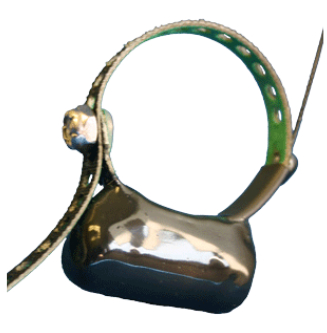
\includegraphics[scale=0.5]{ATS1} & 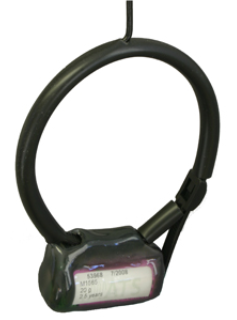
\includegraphics[scale=0.5]{ATS2} & 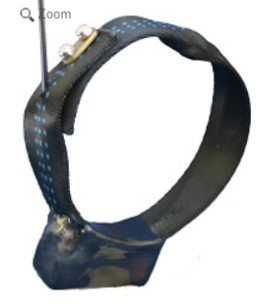
\includegraphics[scale=0.5]{ATS3} \vspace{0.4cm}\\

Peso & 9 a 16g & 10 a 40g & 65 a 115g \vspace{0.4cm}\\

Bateria & Lítio / 156 a 282 dias & Lítio / 195 a 596 dias & AA / 1,75 a 3,5 anos \vspace{0.4cm} \\

Material & 
\makecell{- Coleira de \\ \textbf{neoprene} \\
- Encapsulamento \\ de resina a prova \\ de água} &
\makecell{ - Coleira de \textbf{tubo} \\ \textbf{de plástico (cable-tie)} \\
- Encapsulamento \\ de resina a prova \\ de água} &
\makecell{- Coleira de \textbf{neoprene} \\ \textbf{ou nylon} }   
\end{tabular}
\end{table}

Como visto no item anterior, comercialmente é utilizado rádio na maior parte dos casos (M17X0 e M15X5) e, eventualmente, GPS (W500 - para o qual é possível notar que exige um peso bem superior ao limite estabelecido de cerca de 10g).
\FloatBarrier

\section{Algoritmos}
Inicialmente, é necessário compreender uma forma de calcular a posição dos animais através da distância entre macaco e ponto de acesso. De praxe, em RSSFs este cálculo pode ser feito de duas formas.

A primeira delas é utilizando a intensidade do sinal (\textit{Received Signal Strength Indication} - RSSI). O cálculo da distância, neste caso, é dado pelo seguinte modelo proposto pela Texas Instruments, que é melhor detalhado por Dong e Dargie (2012).

\begin{equation}
RSSI = -10 \times n \times \log_{10} d + A
\end{equation}

Sendo:
\begin{itemize}
\item d a distância em metros
\item RSSI a intensidade do sinal em dBm
\item n a constante de propagação do sinal
\item A a intensidade do sinal para 1 metro de distância
\end{itemize}

Essa é uma maneira simples de baixo custo de implementação, porém, como é bem destacado por Larsson (2015), dada a alta variação de n devido a suscetibilidade do sinal à interferência do meio, demonstra-se um tanto imprecisa.

A constante de propagação pode ser determinada empiricamente. Se sabe n=2 para o vácuo; no ar, valores coerentes estão entre 2.7 e 4. A determinação da constante para este projeto pode ser observada no apêndice.

Outra forma seria calcular a distância sabendo a velocidade de propagação do sinal no meio, dado o tempo que demora para que o sinal seja recebido a partir da implementação de um eco. Idealmente esta é uma abordagem muito mais precisa, que só é impossibilitada em casos que o hardware utilizado não possua relógio. No entanto, qualquer deficiência na temporização e sincronização, por menor que seja, pode comprometer a precisão de tal metodologia.

Para este projeto, pretende-se implementar a primeira forma e verificar a precisão da mesma.

Além disso, foi requerido desenvolver um algoritmo para obtenção do mapeamento da posição dos macacos. Este tema já havia sido discutido por Amaral e Biscaro (2017) e, para este caso, o único algoritmo que se fez praticável é a trilateração.

\begin{figure}[ht]
  \centering
    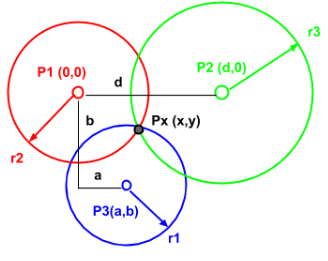
\includegraphics[scale=1]{trilateracao}
  \caption{Algoritmo de trilateração (Fonte: autores)}
\end{figure}
\FloatBarrier

Dada a figura acima, o ponto P pode ser calculado conhecendo-se os pontos fixos P1, P2, P3, as distâncias entre eles e as distâncias entre os mesmos e P (r1, r2 e r3, respectivamente). Assim, é criado um sistema compondo as três equações de circunferências, resultando no seguinte equacionamento.

Se x1 $\neq$ x2:

\quad $\alpha = \dfrac{x1 - x3}{x2 - x1}$

\quad $\beta = 2 \times [(y3 - y1) + \alpha(y2 - y1)]$

\quad Se $\beta \neq$ 0:

\quad \quad y = $\dfrac{(x3^2 - x1^2) + (y3^2 - y1^2) + (r1^2 - r3^2) + \alpha[(x2^2 - x1^2) + (y2^2 - y1^2) + (r1^2 - r2^2)]}{\beta}$

\quad \quad x = $\dfrac{2y(y1 - y2) + (x2^2 - x1^2) + (y2^2 - y1^2) + (r1^2 - r2^2)}{2(x2 - x1)}$

Senão, se x2 $\neq$ x3:

\quad $\alpha = \dfrac{x1 - x3}{x3 - x2}$

\quad $\beta = 2 \times [(y3 - y1) + \alpha(y2 - y3)]$

\quad Se $\beta \neq$ 0:

\quad \quad y = $\dfrac{(x3^2 - x1^2) + (y3^2 - y1^2) + (r1^2 - r3^2) + \alpha[(x3^2 - x2^2) + (y3^2 - y2^2) + (r2^2 - r3^2)]}{\beta}$

\quad \quad x = $\dfrac{2y(y2 - y3) + (x3^2 - x2^2) + (y3^2 - y2^2) + (r2^2 - r3^2)}{2(x3 - x2)}$

Se não couberem nenhum desses dois casos, sabemos que as circunferências não possuem ponto de intersecção,

%\chapter{Metodologia do Trabalho}
Seguindo as orientações de projeto de embarcados indicadas pelo professor orientador (Cugnasca, 2018), inicialmente é necessário levantar e descrever os requisitos funcionais e não funcionais do sistema - o que é feito já no capítulo seguinte.

A segunda etapa consiste na definição da arquitetura do projeto, para qual os possíveis componentes são associados estabelecendo uma composição que cubra os requisitos funcionais do projeto. A arquitetura é descrita no capítulo 6.

A seguir, aos componentes visíveis no plano físico, o que é feito no capítulo 5. Por fim, é implementado a arquitetura que foi projetada.

É adotada metodologia top-down visto que primeiro é definido o produto que se deseja obter para poder segmentar as tarefas a serem realizadas em micro serviços.

Ao mesmo tempo o projeto utiliza duas abordagens. Em alguns aspectos é utilizado o modelo em cascata, pois, por se tratar de um trabalho de formatura, é natural que algumas otimizações sejam reservadas para projetos futuros. Por esse ponto de vista, é como se cada projeto fosse uma curva na espiral.

Por outro lado, dada a abrangência tecnológica do projeto, em frentes como a interface será adotado o modelo espiral, pois neste caso modificações eventuais são menos custosas em tempo e orçamento. Portanto, estão planejados testes de usabilidade do software em diversas etapas de produção.


%\chapter{Especificação de Requisitos de Sistema}
O funcionamento essencial do sistema, o que define seus requisitos funcionais, requer que a posição dos macacos seja possível de ser medida, armazenada e mostrada para o usuário.

Além desses, são levantados os requisitos não funcionais, que trabalham aspectos necessários e complementares para o bom funcionamento do sistema, muitas vezes previstos pelo público solicitante do mesmo.

No SIMIOS, os principais requisitos não funcionais foram apontados por pesquisadores biólogos e veterinários com experiência em monitoramento de macacos. Dentre eles, está que o peso da mochila que será anexada ao animal não deveria ultrapassar 10g para não influenciar em seu comportamento nem sobrecarregá-lo, visto que o principal grupo de foco (saguis) tem peso médio de 400g. Para isso, é interessante que todos os componentes da mochila sejam o mais leves possível.

Outra situação apontada é o fato de que toda vez que a bateria do aparelho tiver de ser trocada, o veterinário deverá capturar o macaco e sedá-lo, o que é bastante prejudicial para a confiança que o animal constrói pelo ser humano. Dessa forma, é desejável que a eficiência energética do dispositivo embarcado seja alta para que a bateria tenha de ser trocada com a menor frequência possível.

Além da mochila do animal, espera-se que os dados coletados sejam confiáveis. Isso envolve garantir a autenticidade e a ausência de erros, ou seja, que eles estejam sendo de fato enviados íntegros pelo macaco a quem estão associados. Assim, evita-se casos em que o dispositivo possa ter sido removido acidentalmente e, por exemplo, enroscado em uma árvore ou em que existam interferências ruidosas no sinal capazes de alterar significativamente as medições enviadas. Também é relevante que o acesso à informação seja possível somente para pessoas autorizadas, envolvendo conceitos como autenticação e codificação.

SIMIOS é um sistema que, estruturalmente, poderia ser contextualizado em praticamente qualquer aplicação que se tenha algo a ser rastreado, seja um ser vivo ou não, para qual a precisão do GPS seja insuficiente. Portanto, de maneira geral, também é interessante que o sistema tenha escalabilidade em todos os aspectos - que os dispositivos embarcados nos animais possuam sensores diversos e que, possivelmente, toda a aplicação suporte que uma quantidade maior de variáveis e de usuários seja inserida.

Por fim, é sempre relevante que a interface com o usuário siga princípios de UX, especialmente se considerando que uma quantidade grande de dados deve ser visualizada de forma intuitiva e simples pelo pesquisador.

\begin{figure}[ht]
  \centering
    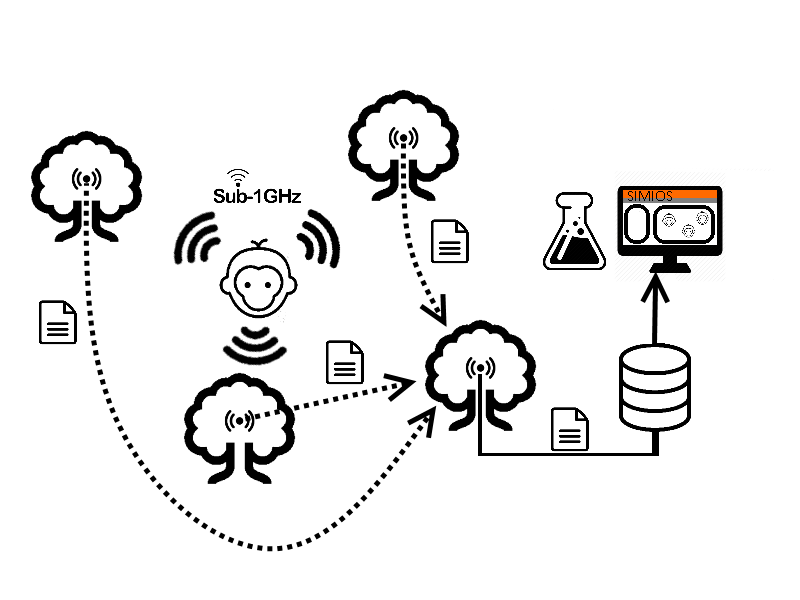
\includegraphics[scale=0.7]{esquematico}
  \caption{Resumo gráfico do sistema (Fonte: autores)}
\end{figure}
\FloatBarrier

%\chapter{Tecnologias Utilizadas}
Considerando os aspectos discutidos no capítulo 2 sobre possíveis e impossíveis instrumentos para o nosso contexto, por fim foram selecionadas as tecnologias que serão efetivamente utilizados no projeto, as quais são descritas neste capítulo.

\section{Dispositivo Embarcado}
Partindo disso, selecionou-se a plataforma de desenvolvimento do Sensor Tag da Texas Instruments como componente embarcado de cada macaco. Trata-se de uma placa leve que contém 6 sensores, incluindo de temperatura, e comunicador BLE. Seu datasheet pode ser encontrado nas referências deste trabalho.

\begin{figure}[ht]
  \centering
    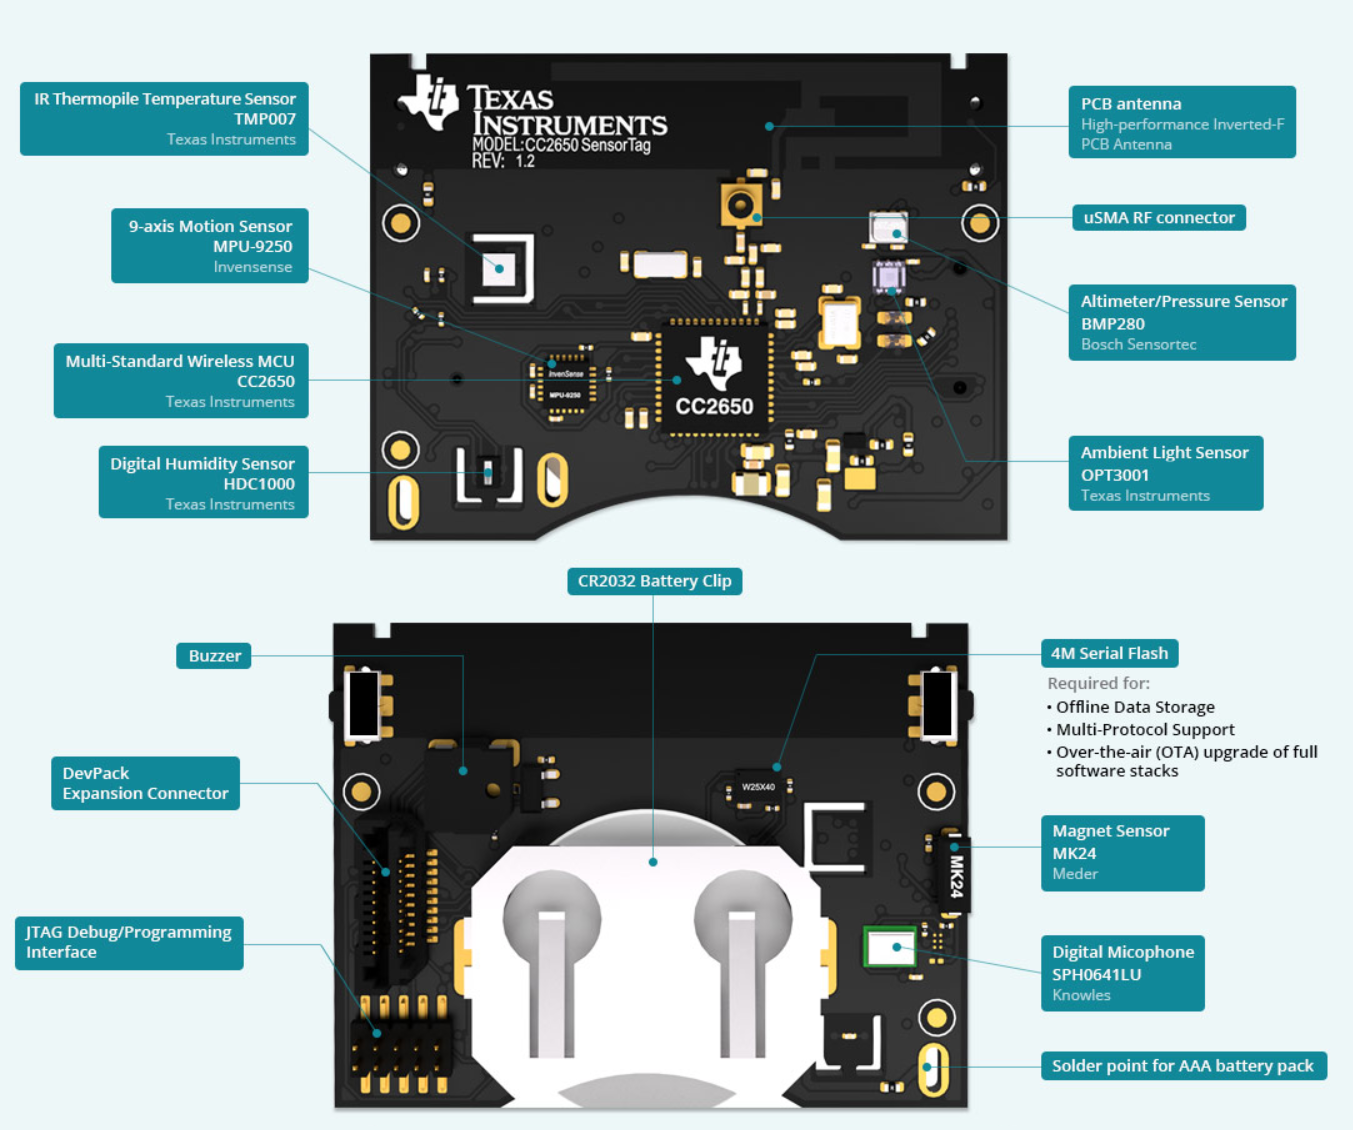
\includegraphics[scale=0.5]{sensortag}
  \caption{Componentes do Sensor Tag (Fonte: extraído do site da Texas Instruments)}
\end{figure}

Foi utilizado um Raspberry Pi 2 para receber por BLE os dados de cada Sensor Tag e enviá-los por Wi-fi para o servidor, que pode ser local ou em nuvem. 

\section{Servidor}
Foi escolhido o banco de dados relacional MySQL da Oracle por se tratar de um sistema open source simples, embora completo.

O projeto SIMIOS prevê o rastreio de animais em reservas, o que envolve, como visto anteriormente, no máximo cerca de 50 animais em grandes reservas. Dessa forma, sabemos que não envolve sobrecarga de acessos por segundo e mesmo isto poderia ser corrigido com buffering.

Um ponto negativo do MySQL é que sua escalabilidade pode ser prejudicada - cada servidor tem um tamanho limitado e cada set de dados só pode ser alocado em um servidor (não suporta particionamento), o que pode ser prejudicial em casos que deseja-se guardar no banco grande quantidade de dados. Para corrigir tal empecilho é possível implementar importação de dados.

\section{Software}
Para desenvolvimento do programa computacional que é executado no servidor, foi escolhida a linguagem de programação Java, com suporte de frameworks Spring e JPA, facilitando principalmente os processos de queries do banco de dados, de autenticação e autorização e de mapeamento de interface model-view-controller (MVC).

Por se tratar de uma aplicação de histórico de dados, pouquíssimo processamento está previsto e a computação pode ser realizada em tempo real pelo computador do usuário. Dessa forma, não se faz necessário o uso de linguagem de programação de execução eficiente (C++, por exemplo).


\include{projeto-implementacao}

\include{testes-avaliacao}

\include{consideracoes-finais}

% ========== Referências ==========
% --- IEEE ---
%	http://www.ctan.org/tex-archive/macros/latex/contrib/IEEEtran
\bibliographystyle{IEEEbib}

% --- ABNT (requer ABNTeX 2) ---
%	http://www.ctan.org/tex-archive/macros/latex/contrib/abntex2
%\bibliographystyle{abntex2-num}

\bibliography{}


% ========== Apêndices (opcional) ==========
\apendice
\chapter{}
\chapter{Beta}


% ========== Anexos (opcional) ==========
\anexo
\chapter{Alpha}
\chapter{}



\end{document}
